\section{XML} 

  So far, we have talked about relational data, which is a type of \textbf{structured data} with a schema, attributes, tuples, etc along with their types and constraints. For example, just trying to add a new attribute to a relation may require you to add the attribute for each tuple if it cannot be null. Some \textbf{unstructured data} is just plaintext, which doesn't confirm to any schema, and is on the other extreme end. Some types of data in between is HTML, XML, or JSON, which we call \textbf{semi-structured}, which may contain sections, subsections, etc. 

  \begin{definition}[XML]
    The \textbf{extensible markup language (XML)} is a semi-structured data that is similar to HTML, where the data self-describes the structure.\footnote{The names and nesting of its tags describe its structure.} 
    \begin{enumerate}
      \item There are \textbf{tags} marked by a start (\texttt{<tag>}) and end (\texttt{</tag>}) tags. 
      \item An \textbf{element} is enclosed by a pair of start and end tags(\texttt{<t>...</t>}), and elements can be nested (\texttt{<t><r></r></t>}or empty(\texttt{<t></t>}.  
      \item Elements can also have \textbf{attributes} (\texttt{<book ISBN="...", price="80.00">}).\footnote{This is not the same attributes in relational databases.} Attributes must be unique, i.e. there cannot be duplicate attributes in a tag. 
    \end{enumerate}
    Note that there are some conventions that we must follow to get a \textbf{well-formed} XML document. First, the tags should be closed appropriately like parantheses matching, and we should not have the characters \texttt{<} or \texttt{>} as a part of the element. Rather, we should use \texttt{\&lt;} and \texttt{\&gt;}. 
  \end{definition}

  \begin{example}
    An example of XML data regarding a book is 
    \begin{lstlisting}
      <?xml version="1.0" encoding="UTF-8"?>
      <book>
          <title>The Great Gatsby</title>
          <author>
              <firstName>F. Scott</firstName>
              <lastName>Fitzgerald</lastName>
          </author>
          <published>
              <year>1925</year>
              <publisher>Charles Scribners Sons</publisher>
          </published>
          <genre>Literary Fiction</genre>
          <price currency="USD">14.99</price>
          <inStock>true</inStock>
          <rating>4.5</rating>
      </book> 
    \end{lstlisting}
    This can be represented by a tree. 

    \begin{figure}[H]
      \centering 
      \begin{tikzpicture}[
        scale=0.75,
        transform shape,
        level 1/.style={sibling distance=70mm},
        level 2/.style={sibling distance=23mm},
        level 3/.style={sibling distance=22mm},
        every node/.style={
          draw, 
          ellipse, 
          minimum height=0.7cm, 
          align=center
        }
        ]
        % Root node
        \node {bibliography}
          % Level 1
          child { node (book1) {book}
            % Level 2 - first book's elements
            child { node {title} 
              child { node[draw=none] {Foundations\\of Databases} }
            }
            child { node {author}
              child { node[draw=none] {Abiteboul} }
            }
            child { node {author}
              child { node[draw=none] {Vianu} }
            }
            child { node {publisher}
              child { node[draw=none] {Addison\\Wesley} }
            }
            child { node {year}
              child { node[draw=none] {1995} }
            }
            child[xshift=30mm] { node {section}
              % Level 3 - section elements
              child { node {title}
                child { node[draw=none] {Introduction} }
              }
              child { node {content}
                child { node[draw=none, align=left] {In this\\section...} }
              }
              child { node {section} }
              child { node {section} }
            }
          }
          child { node {book} }
        ;
      \end{tikzpicture}
      \caption{Tree representation of an XML file.} 
      \label{fig:tree_rep}
    \end{figure}
  \end{example}


  Let's do a quick comparison of relations and XML. 
  \begin{enumerate}
    \item One advantage of XML is portability/exchangeability, since it self-describes itself, so all you really need is this text, unlike relations where you should also send the schema and other metadata. On the other hand, exchanging is problematic. 
    \item Second, its has flexibility to represent any information (e.g. structured, semi-structured, documents, etc.). Unlike a relation where each attribute of each tuple is atomic (meaning you can't place another relation in there), you can make a new XML tree. 
    \item Finally, since the data describes itself, you can change the schema easily. In contrast, the schema of a relational database is always fixed in advance and difficult to change. 
    \item Almost all major DBMS supports relations, and XML is often implemented as an add-on on top of relations. 
    \item Unlike the relational database where the order of the rows don't matter, the order does matter for XML. 
  \end{enumerate}
  
  \begin{definition}[DTD]
    Just because we don't need metadata does not mean that we cannot define one. This is done with the \textbf{document type definitions (DTD)}, which species the schema and constraints for XML just like relational databases. It has the following syntax, which should be written in the beginning of the XML file. 
    \begin{lstlisting}
      <!DOCTYPE root-element [
         <!ELEMENT element-name (content-specification)>
      ]> 
    \end{lstlisting} 
    Here are the common element specifications. 
    \begin{enumerate}
      \item \texttt{EMPTY}: Element has no content
      \item \texttt{ANY}: Element can contain any content
      \item \texttt{(\#PCDATA)}: Element contains parsed character data
      \item \texttt{Child elements}: Listed in parentheses
    \end{enumerate}
    with an example of a simple DTD being 
    \begin{lstlisting}
      <!DOCTYPE library [
         <!ELEMENT library (book+)>
         <!ELEMENT book (title, author, year)>
         <!ELEMENT title (#PCDATA)>
         <!ELEMENT author (#PCDATA)>
         <!ELEMENT year (#PCDATA)>
      ]> 
    \end{lstlisting}
  \end{definition}

  Really, this is like a tree directory structure, so to query data, it makes sense to try and traverse the paths. There are three major query languages for XML, which are 
  \begin{enumerate}
    \item \textbf{XPath}, which uses path expressions with conditions and are the building blocks of the rest of the standards. 
    \item \textbf{XQuery}, which is XPath plus a full-fledged SQL-like query language. 
    \item \textbf{XSLT}, or eXtensible Stylesheet Language Transformations and is the recommended style sheet language for XML. 
  \end{enumerate}

\subsection{XPath}

  \begin{definition}[Basic XPath Constructs]
    The syntax for building a XPath is as follows: 
    \begin{enumerate}
      \item \texttt{/}: used as a separator between steps in a path (traversing down). 
      \item \texttt{name}: matches any child element with this tag name. 
      \item \texttt{*}: matches any child element 
      \item \texttt{@name}: matches the attribute with this name. 
      \item \texttt{@*}: matches any attribute 
      \item \texttt{//}: matches any descendent element of the current element itself. 
      \item \texttt{. }: matches current element.
      \item \texttt{.. }: matches parent element.\footnote{This is just like when we are navigating directories in a shell.}
    \end{enumerate}
    Note that these names are all case sensitive, and another important fact is that NULL evaluates to NOT (so if there are no elements/attributes), then a condition on that element/attribute will evaluate to NOT. 
  \end{definition}

  \begin{example}
    Let's look at this example, which shows bibliographies for different books. 
    \begin{lstlisting}
      <?xml version="1.0" encoding="UTF-8"?>
      <bibliography>
          <book ISBN="ISBN-10" price="70">
              <title>Foundations of Databases</title>
              <author>Abiteboul</author>
              <author>Hull</author>
              <author>Vianu</author>
              <publisher>Addison Wesley</publisher>
              <year>1995</year>
              <section>abc</section>
          </book>
          <book ISBN="ISBN-11" price="20">
              <title>DBSTS</title>
              <author>Ramakrishnan</author>
              <author>Gehrke</author>
              <publisher>Addison Wesley</publisher>
              <year>1999</year>
              <section>
                <title>bruh</title>
              </section>
          </book>
          <report>
            <author>Muchang</author>
            <addon>
              <author>Jon</author>
            </addon>
          </report>
      </bibliography> 
    \end{lstlisting}
    Let's look at some XPaths. 
    \begin{enumerate}
      \item \texttt{/bibliography/book/author} gets all author element reachable via this path.
        \begin{lstlisting}
          <author>Abiteboul</author>
          <author>Hull</author>
          <author>Vianu</author>
          <author>Ramakrishnan</author>
          <author>Gehrke</author>
        \end{lstlisting}

      \item \texttt{/bibliography/book/title} gets all book titles reachable via this path. 
        \begin{lstlisting}
          <title>Foundations of Databases</title>
          <title>DBSTS</title>
        \end{lstlisting}

      \item \texttt{/bibliography/book/@ISBN} gets all book ISBN attributes (we need the \texttt{\@} to search the \textit{attribute}, not the element)
        \begin{lstlisting}
          ISBN="70"
          ISBN="ISBN:11"
        \end{lstlisting}

      \item \texttt{//title} returns all title elements, anywhere in the document. Note that the title of the section is also added. 
        \begin{lstlisting}
          <title>Foundations of Databases</title>
          <title>DBSTS</title>
          <title>bruh</title>
        \end{lstlisting}

      \item \texttt{//section/title} returns all section titles, anywhere in the document.
        \begin{lstlisting}
          <title>bruh</title>
        \end{lstlisting}

      \item \texttt{/bibliography/*/author} returns all authors in bibliography that is a grandchild of bibliography. Note that Muchang is retrieved but not Jon. 
        \begin{lstlisting}
          <author>Abiteboul</author>
          <author>Hull</author>
          <author>Vianu</author>
          <author>Ramakrishnan</author>
          <author>Gehrke</author>
          <author>Muchang</author>
        \end{lstlisting}

      \item \texttt{/bibliography/book[@price<50]} returns all books that are children of bibliography with attribute price less than 50. 
        \begin{lstlisting}
          <book ISBN="ISBN-11" price="20">
              <title>DBSTS</title>
              <author>Ramakrishnan</author>
              <author>Gehrke</author>
              <publisher>Addison Wesley</publisher>
              <year>1999</year>
              <section>
                <title>bruh</title>
              </section>
          </book>
        \end{lstlisting}

      \item \texttt{/bibliography/book[author='Abiteboul']} returns all books that are children of bibliography that has an author tag children with element Abiteboul. 

      \item \texttt{/bibliography/book[author]} returns all books that are children of bibliography with some child author tag. 

      \item \texttt{/bibliography/book[40 <= @price and @price <= 50]} returns books with price attribute between 40 and 50. 

      \item \texttt{/bibliography/book[author='Abiteboul' or @price >=50]} returns books either authored by Abiteboul or price at least 50. Note that the first condition is on an element and the second is on an attribute. 

      \item \texttt{/bibliography/book[author='Abiteboul' or not (@price < 50)]} returns books authored by Abiteboul or price not below 50. Note that this is different from the query above since if a book does not have a price, then \texttt{\@price < 50} is null (which is NOT in XPath), so it returns the book. 
    \end{enumerate}
  \end{example}

  Hopefully you get a good feel for how XPaths work. Here's a trickier example. 

  \begin{example}[Conditions on Any vs All Attributes/Elements]
    Say you want to get all books with some price in the range $[20, 50]$. Then you would think of writing 
    \begin{lstlisting}
      /bibliography/book/[price>=20 and price <=50]
    \end{lstlisting}
    This may not work if we have a XML element of this form, with multiple prices. 
    \begin{lstlisting}
      <book> 
        <title>newbooktitle</title>
        <price>10</price>
        <price>70</price> 
      </book>
    \end{lstlisting} 
    since it compares is any element satisfies the conditions. Therefore, we can think of these conditions all as the \texttt{any} condition over child elements. If we want to use the \texttt{all} condition, we can write 
    \begin{lstlisting}
      /bibliography/book/[price[.>=20 and .<=50]]
    \end{lstlisting}

    Similarly, if we have the query \texttt{/bibliography/book[author='A' and author!='A']}, this is an any clause, so it will return all books with author A and another author not A. 
  \end{example}

  \begin{definition}[XPath Operators and Functions] 
    In conditions, we can use the following operations. 
    \begin{enumerate}
      \item Arithmetic: \texttt{x + y}, \texttt{x - y}, \texttt{x * y}, \texttt{x div y}, \texttt{x mod y} 
      \item \texttt{contains(x, y)} returns true if string \texttt{x} contains string \texttt{y} 
      \item \texttt{count(node-set)} counts the number of nodes in \texttt{node-set} 
      \item \texttt{position()} returns the \textit{context position} (i.e the position of the node amongst its siblings) 
      \item \texttt{last()} returns the \textit{context size} (roughly the size of the node-set)
      \item \texttt{name()} returns the tag name of the current element
    \end{enumerate}
  \end{definition}

  \begin{example}
    Some more queries is 
    \begin{enumerate}
      \item \texttt{/bibliography/book[count(section)<10]} returns books with fewer than 10 sections. 
      \item \texttt{//*[contains(name(), 'Ab')]} returns all elements whose tag names contain \texttt{Ab} (or \texttt{section}?) 
      \item \texttt{/bibliography/book/section[position()=1]/title} returns the title of the first section in each book. 
      \item \texttt{/bibliography/book/section[position()=last()]/title} returns the title of the last section in each book.
    \end{enumerate}
  \end{example}

\subsection{XQuery}
  
  XQuery is a superset of the XPath, but it also encompasses FLWOR  expressions, quantified expressions, aggregation, sorting, etc. An XQuery expression can even return a new result XML document. Let's put the XML example file again for convenience. 

  \begin{lstlisting}
    <?xml version="1.0" encoding="UTF-8"?>
    <bibliography>
        <book ISBN="ISBN-10" price="70">
            <title>Foundations of Databases</title>
            <author>Abiteboul</author>
            <author>Hull</author>
            <author>Vianu</author>
            <publisher>Addison Wesley</publisher>
            <year>1995</year>
            <section>abc</section>
        </book>
        <book ISBN="ISBN-11" price="20">
            <title>DBSTS</title>
            <author>Ramakrishnan</author>
            <author>Gehrke</author>
            <publisher>Addison Wesley</publisher>
            <year>1999</year>
            <section>
              <title>bruh</title>
            </section>
        </book>
    </bibliography> 
  \end{lstlisting}

  \begin{example}
    For now, let's start with a simple XQuery based on XPath. To find all books, we can write the following, where the first \texttt{doc} refers to the specific document to query.
    \begin{lstlisting}
      <result>{
        doc("bib.xml")/bibliography/book
      }</result>
    \end{lstlisting}
    Note that like Python string interpolation, text outside of \texttt{\{\}} are copied to output verbatim, while those inside are evaluated and replaced by the result. We can use conditionals the same way. 
    \begin{lstlisting}
      <result>{
        doc("bib.xml")/bibliography/book[@price<50]
      }</result>
    \end{lstlisting}
    which will return 
    \begin{lstlisting}
      <book ISBN="ISBN-11" price="20">
          <title>DBSTS</title>
          <author>Ramakrishnan</author>
          <author>Gehrke</author>
          <publisher>Addison Wesley</publisher>
          <year>1999</year>
          <section>
            <title>bruh</title>
          </section>
      </book>
    \end{lstlisting}
  \end{example}

  \begin{definition}[FLWOR Expressions]
    The fundamental building block of XQuery is the FLWOR expression, which stands for:
    \begin{enumerate}
      \item \texttt{FOR}: Iterates over sequences
      \item \texttt{LET}: Binds variables to values
      \item \texttt{WHERE}: Filters the tuples
      \item \texttt{ORDER BY}: Sorts the results
      \item \texttt{RETURN}: Constructs the result
    \end{enumerate}
    Note that only the \texttt{RETURN} clause is mandatory; all others are optional.
  \end{definition}

  \begin{example}[FLWOR with Loops and Conditionals]
    To retreive the titles of books published before 2000, together with their publisher, we can write either of the following. The logic is pretty self explanatory. 

    \noindent\begin{minipage}{.5\textwidth}
    \begin{lstlisting}[]{Code}
      <result>{
        for $b in /bibliography/book 
        let $p := $b/publisher 
        where $b/year < 2000 
        return 
          <book>
          { $b/title }
          { $p }
          </book>
      }</result>
    \end{lstlisting}
    \end{minipage}
    \hfill
    \begin{minipage}{.49\textwidth}
    \begin{lstlisting}[]{Output}
      <result>{
        for $b in /bibliography/book[year<2000]
        return 
          <book>
          { $b/title }
          { $p/publisher }
          </book>
      }</result>
      .
      .
    \end{lstlisting}
    \end{minipage}
    which will return 
    \begin{lstlisting}
      <result>
        <book>
          <title>Foundations of Databases</title>
          <publisher>Addison Wesley</publisher>
        </book>
        <book>
          <title>DBSTS</title>
          <publisher>Addison Wesley</publisher>
        </book>
      </result> 
    \end{lstlisting}
    Note that \texttt{\$p} may be assigned to a set of elements. It does not have to be one element. 
  \end{example}

  Just like XPath, a conditional expression (with where) only checks the \texttt{any} condition. 
  
  \begin{example}[Nested Loops and List Comprehension]
    We can also use nested loops to solve the query above, but note the logic. If a book of price < 2000 has 2 publishers, then the book may be returned 2 times. On the other hand, if a book has a price < 2000 but has no publishers, then a null is really a false, so that book will not be returned. 

    \noindent\begin{minipage}{.5\textwidth}
      \begin{lstlisting}[]{Code}
        <result>
        {
          for $b in /bibliography/book,
          $p in $b/publisher
          where $b/year < 2000
          return 
            <book>{ $b/title }{ $p }</book>
        }
        </result> 
        .
        .
        .
        .
        .
      \end{lstlisting}
      \end{minipage}
      \hfill
      \begin{minipage}{.49\textwidth}
      \begin{lstlisting}[]{Output}
        <result>
          <book>
            <title>Foundations of Databases</title>
            <publisher>Addison Wesley</publisher>
          </book>
          <book>
            <title>Foundations of Databases</title>
            <publisher>Springer</publisher>
          </book>
          <book>
            <title>DBSTS</title>
            <publisher>Addison Wesley</publisher>
          </book>
        </result>          
      \end{lstlisting}
    \end{minipage}

    If we use a comprehension statement, we can let \texttt{\$b} be all the books and try to parse them element by element where its year is < 2000. This is also wrong since the where clause is an any expression, so if at least 2 book has year < 2000, then it will return all the books. In fact, it doesn't even return it in the right format, since it returns all the book titles first and then all the publishers. 

    \noindent\begin{minipage}{.5\textwidth}
      \begin{lstlisting}[]{Code}
        <result>
        {
          let $b := /bibliography/book
          where $b/year < 2000
          return 
            <book>
              { $b/title }
              { $b/publisher }
            </book>
        }
        </result>          
      \end{lstlisting}
      \end{minipage}
      \hfill
      \begin{minipage}{.49\textwidth}
      \begin{lstlisting}[]{Output}
        <result>
          <book>
            <title>Found of Databases</title>
            <title>DBSTS</title>
            <publisher>Addison Wesley</publisher>
          </book>
        </result>
        .
        .
        .
        .
      \end{lstlisting}
    \end{minipage}
  \end{example}

  Now that we went over FLWOR, let's talk about how we can do joins. 

  \begin{example}[Explicit Join]
    To find all pairs of books that have common authors, we can write 
    \begin{lstlisting}
      <result>
      {
        for $b1 in //book
        for $b2 in //book
        where $b1/author = $b2/author
        and $b1/title > $b2/title
        return
          <pair>
            { $b1/title }
            { $b2/title }
          </pair>
      }
      </result> 
    \end{lstlisting}
    Remember that since the where is an any condition, this works to our advantage now. We also use a string comparison of the authors and titles to remove duplicates. This gives us the result. 
    \begin{lstlisting}
      <result>
        <pair>
          <title>Foundations of Databases</title>
          <title>DBSTS</title>
        </pair>
      </result> 
    \end{lstlisting}
  \end{example}

  We will stop here, but there are more features such as subqueries, existential (some) vs universal (all) queries, aggregation, conditional, etc. 

\subsection{Converstion of XML to Relational Data} 
  
  Relational to XML is trivial, but XML to relational isn't really since there can be different data types that are siblings (e.g. books vs articles, vs papers all under bibliography), there may be repeats of the same tag, and there are both child elements and attributes. 
  
  The most trivial thing to do is to store the entire XML in a column (called a CLOB, character large Object type), but this isn't useful since it first does not satisfy the condition that each element must be atomic in a relation. There are two alternatives. 
  \begin{enumerate}
    \item \textbf{Schema-Oblivious Mapping} takes a well-formed XML and converts it to a generic relational schema. In here, there are more subtypes. 
      \begin{enumerate}
        \item \textbf{Node/edge based mapping} for graphs. 
        \item \textbf{Interval based mapping} for trees.
        \item \textbf{Path based mapping} for trees. 
      \end{enumerate}
    \item \textbf{Schema-Aware Mapping} takes a valid XML and converts it to a special relational schema based on DTD. 
  \end{enumerate} 

  Let's go over the node/edge based mapping. This is quite intuitive since we can visualize a XML structure as a directed graph. 

  \begin{figure}[H]
    \centering
    \begin{subfigure}[b]{0.58\textwidth}
      \centering
      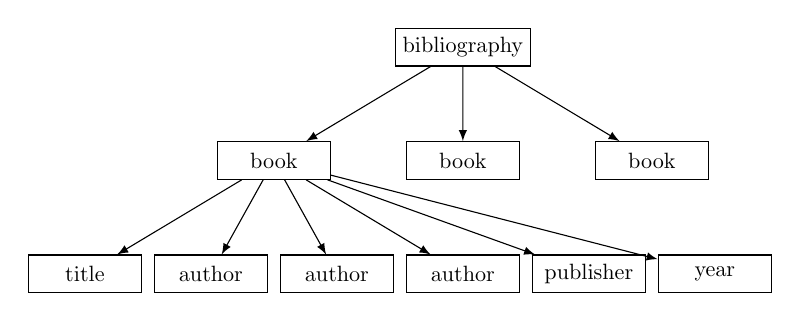
\begin{tikzpicture}[
          level 1/.style={sibling distance=2.5cm},
          level 2/.style={sibling distance=1.5cm},
          every node/.style={
            draw,
            rectangle,
            font=\normalfont,
            minimum height=0.6cm, 
            minimum width=1.8cm,
            text centered
          },
          scale=0.8,
          transform shape
        ]
        % Root node
        \node (bibliography) at (0,0) {bibliography};
          
        % Level 1 nodes (books)
        \node (book1) at (-3,-1.8) {book};
        \node (book2) at (0,-1.8) {book};
        \node (book3) at (3,-1.8) {book};
        
        % Level 2 nodes (book elements)
        \node (title) at (-6,-3.6) {title};
        \node (author1) at (-4,-3.6) {author};
        \node (author2) at (-2,-3.6) {author};
        \node (author3) at (0,-3.6) {author};
        \node (publisher) at (2,-3.6) {publisher};
        \node (year) at (4,-3.6) {year};
        
        % Draw arrows from bibliography to books
        \draw[-latex] (bibliography) -- (book1);
        \draw[-latex] (bibliography) -- (book2);
        \draw[-latex] (bibliography) -- (book3);
        
        % Draw arrows from book1 to its elements
        \draw[-latex] (book1) -- (title);
        \draw[-latex] (book1) -- (author1);
        \draw[-latex] (book1) -- (author2);
        \draw[-latex] (book1) -- (author3);
        \draw[-latex] (book1) -- (publisher);
        \draw[-latex] (book1) -- (year);
      \end{tikzpicture}
      \caption{XML document hierarchy as a tree structure}
      \label{fig:xml-tree}
    \end{subfigure}
    \hfill 
    \begin{subfigure}[b]{0.40\textwidth}
      \centering
      \begin{lstlisting}
        <bibliography>
        <book ISBN="ISBN-10" price="80.00">
        <title>Databases</title>
        <author>Abiteboul</author>
        <author>Hull</author>
        <author>Vianu</author>
        <publisher>Addison </publisher>
        <year>1995</year>
        </book>
        </bibliography>
      \end{lstlisting}
      \caption{XML document code representation}
      \label{fig:xml-code}
    \end{subfigure}
    \caption{Two representations of an XML document: hierarchical tree structure (left) and code format (right)}
    \label{fig:xml-representations}
  \end{figure}

  We can convert the XML to the following 4 relations. We also put the bibliography example to make it easier to follow along. 
  \begin{enumerate}
    \item \textbf{Element(\underline{eid}, tag)}. All elements will have a certain id with their tag type. Note that elements can have text inside of them, but we will consider this a ``child'' of the element, stored in the \texttt{Text} relation. 

      \begin{table}[H]
        \centering
        \caption{Element Table}
        \begin{tabular}{|l|l|}
          \hline
          \textbf{eid} & \textbf{tag} \\
          \hline
          e0 & bibliography \\
          e1 & book \\
          e2 & title \\
          e3 & author \\
          e4 & author \\
          e5 & author \\
          e6 & publisher \\
          e7 & year \\
          \hline
        \end{tabular}
        \caption{}
        \label{tab:}
      \end{table}

    \item \textbf{Attribute(eid, attrName, attrValue)}. All attributes will need to have their name and type, along with which eid that they are a part of. Note that there is only one functional dependency \texttt{(eid, attrName) -> attrValue}.

      \begin{table}[H]
        \centering
        \caption{Attribute Table}
        \begin{tabular}{|l|l|l|}
        \hline
        \textbf{eid} & \textbf{attrName} & \textbf{attrValue} \\
        \hline
        e1 & ISBN & ISBN-10 \\
        e1 & price & 80 \\
        \hline
        \end{tabular}
      \end{table}

    \item \textbf{ElementChild(eid, pos, child)}. Each element will have a children, with pos referring to the position of the children. Child references either \texttt{Element(eid)} or \texttt{Text(tid)}. 

      \begin{table}[H]
        \centering
        \caption{ElementChild Table}
        \begin{tabular}{|l|l|l|}
        \hline
        \textbf{eid} & \textbf{pos} & \textbf{child} \\
        \hline
          e0 & 1 & e1 \\
          e1 & 1 & e2 \\
          e1 & 2 & e3 \\
          e1 & 3 & e4 \\
          e1 & 4 & e5 \\
          e1 & 5 & e6 \\
          e1 & 6 & e7 \\
          e2 & 1 & t0 \\
          e3 & 1 & t1 \\
          e4 & 1 & t2 \\
          e5 & 1 & t3 \\
          e6 & 1 & t4 \\
          e7 & 1 & t5 \\
        \hline
        \end{tabular}
      \end{table}

    \item \textbf{Text(\underline{tid}, value)}. All text in an element, with an id value (which cannot be the same as any eid) and the actual text in the value. 

      \begin{table}[H]
        \centering
        \caption{Text Table}
        \begin{tabular}{|l|l|}
        \hline
        \textbf{tid} & \textbf{value} \\
        \hline
        t0 & Foundations of Databases \\
        t1 & Abiteboul \\
        t2 & Hull \\
        t3 & Vianu \\
        t4 & Addison Wesley \\
        t5 & 1995 \\
        \hline
        \end{tabular}
      \end{table}
  \end{enumerate}
  Note that we need to invent a lot of ids and need indices for efficiency. 


  Given this, we can write the equivalent SQL queries from these XPath queries. 
  \begin{enumerate}
    \item \texttt{//title} 
      \begin{lstlisting}
        SELECT eid FROM Element WHERE tag='title';
      \end{lstlisting}

    \item \texttt{//section/title} 
      \begin{lstlisting}
        SELECT e2.eid 
        FROM Element e1, ElemtnChild c, Element e2 
        WHERE e1.tag = 'section' 
        AND e2.tag = 'title' 
        AND e1.eid = c.eid 
        AND c.child = e2.eid;
      \end{lstlisting}
      Therefore, path expression becomes joins. The number of joins is proportional to the length of the path expression. 
  \end{enumerate}

